%%%%%%%%%%%%%%%%%%%%%%%%%%%%%%%%%%%%%%%%%
% Beamer Presentation
% LaTeX Template
% Version 2.0 (March 8, 2022)
%
% This template originates from:
% https://www.LaTeXTemplates.com
%
% Author:
% Vel (vel@latextemplates.com)
%
% License:
% CC BY-NC-SA 4.0 (https://creativecommons.org/licenses/by-nc-sa/4.0/)
%
%%%%%%%%%%%%%%%%%%%%%%%%%%%%%%%%%%%%%%%%%

%----------------------------------------------------------------------------------------
%	PACKAGES AND OTHER DOCUMENT CONFIGURATIONS
%----------------------------------------------------------------------------------------

\documentclass[
10pt, % Set the default font size, options include: 8pt, 9pt, 10pt, 11pt, 12pt, 14pt, 17pt, 20pt
%t, % Uncomment to vertically align all slide content to the top of the slide, rather than the default centered
%aspectratio=169, % Uncomment to set the aspect ratio to a 16:9 ratio which matches the aspect ratio of 1080p and 4K screens and projectors
]{beamer}

\graphicspath{{Images/}{./}} % Specifies where to look for included images (trailing slash required)

\usepackage{booktabs} % Allows the use of \toprule, \midrule and \bottomrule for better rules in tables

%----------------------------------------------------------------------------------------
%	SELECT LAYOUT THEME
%----------------------------------------------------------------------------------------

% Beamer comes with a number of default layout themes which change the colors and layouts of slides. Below is a list of all themes available, uncomment each in turn to see what they look like.

%\usetheme{default}
%\usetheme{AnnArbor}
%\usetheme{Antibes}
%\usetheme{Bergen}
%\usetheme{Berkeley}
%\usetheme{Berlin}
%\usetheme{Boadilla}
\usetheme{CambridgeUS}
%\usetheme{Copenhagen}
%\usetheme{Darmstadt}
%\usetheme{Dresden}
%\usetheme{Frankfurt}
%\usetheme{Goettingen}
%\usetheme{Hannover}
%\usetheme{Ilmenau}
%\usetheme{JuanLesPins}
%\usetheme{Luebeck}
%\usetheme{Madrid}
%\usetheme{Malmoe}
%\usetheme{Marburg}
%\usetheme{Montpellier}
%\usetheme{PaloAlto}
%\usetheme{Pittsburgh}
%\usetheme{Rochester}
%\usetheme{Singapore}
%\usetheme{Szeged}
%\usetheme{Warsaw}

%----------------------------------------------------------------------------------------
%	SELECT COLOR THEME
%----------------------------------------------------------------------------------------

% Beamer comes with a number of color themes that can be applied to any layout theme to change its colors. Uncomment each of these in turn to see how they change the colors of your selected layout theme.

%\usecolortheme{albatross}
%\usecolortheme{beaver}
%\usecolortheme{beetle}
%\usecolortheme{crane}
%\usecolortheme{dolphin}
%\usecolortheme{dove}
%\usecolortheme{fly}
%\usecolortheme{lily}
%\usecolortheme{monarca}
%\usecolortheme{seagull}
%\usecolortheme{seahorse}
%\usecolortheme{spruce}
%\usecolortheme{whale}
%\usecolortheme{wolverine}

%----------------------------------------------------------------------------------------
%	SELECT FONT THEME & FONTS
%----------------------------------------------------------------------------------------

% Beamer comes with several font themes to easily change the fonts used in various parts of the presentation. Review the comments beside each one to decide if you would like to use it. Note that additional options can be specified for several of these font themes, consult the beamer documentation for more information.

\usefonttheme{default} % Typeset using the default sans serif font
%\usefonttheme{serif} % Typeset using the default serif font (make sure a sans font isn't being set as the default font if you use this option!)
%\usefonttheme{structurebold} % Typeset important structure text (titles, headlines, footlines, sidebar, etc) in bold
%\usefonttheme{structureitalicserif} % Typeset important structure text (titles, headlines, footlines, sidebar, etc) in italic serif
%\usefonttheme{structuresmallcapsserif} % Typeset important structure text (titles, headlines, footlines, sidebar, etc) in small caps serif

%------------------------------------------------

%\usepackage{mathptmx} % Use the Times font for serif text
%\usepackage{palatino} % Use the Palatino font for serif text

%\usepackage{helvet} % Use the Helvetica font for sans serif text
%\usepackage[default]{opensans} % Use the Open Sans font for sans serif text
%\usepackage[default]{FiraSans} % Use the Fira Sans font for sans serif text
%\usepackage[default]{lato} % Use the Lato font for sans serif text

%----------------------------------------------------------------------------------------
%	SELECT INNER THEME
%----------------------------------------------------------------------------------------

% Inner themes change the styling of internal slide elements, for example: bullet points, blocks, bibliography entries, title pages, theorems, etc. Uncomment each theme in turn to see what changes it makes to your presentation.

\useinnertheme{default}
%\useinnertheme{circles}
%\useinnertheme{rectangles}
%\useinnertheme{rounded}
%\useinnertheme{inmargin}

%----------------------------------------------------------------------------------------
%	SELECT OUTER THEME
%----------------------------------------------------------------------------------------

% Outer themes change the overall layout of slides, such as: header and footer lines, sidebars and slide titles. Uncomment each theme in turn to see what changes it makes to your presentation.

\useoutertheme{default}
%\useoutertheme{infolines}
%\useoutertheme{miniframes}
%\useoutertheme{smoothbars}
%\useoutertheme{sidebar}
%\useoutertheme{split}
%\useoutertheme{shadow}
%\useoutertheme{tree}
%\useoutertheme{smoothtree}

%\setbeamertemplate{footline} % Uncomment this line to remove the footer line in all slides
%\setbeamertemplate{footline}[page number] % Uncomment this line to replace the footer line in all slides with a simple slide count

%\setbeamertemplate{navigation symbols}{} % Uncomment this line to remove the navigation symbols from the bottom of all slides

%----------------------------------------------------------------------------------------
%	PRESENTATION INFORMATION
%----------------------------------------------------------------------------------------

\title[Short Title]{Full Presentation Title} % The short title in the optional parameter appears at the bottom of every slide, the full title in the main parameter is only on the title page

\subtitle{Optional Subtitle} % Presentation subtitle, remove this command if a subtitle isn't required

\author[James Cook \and Roald Amundsen]{Capt. James Cook \and Roald Amundsen} % Presenter name(s), the optional parameter can contain a shortened version to appear on the bottom of every slide, while the main parameter will appear on the title slide

\institute[UC]{the University of Cambridge \\ \smallskip \textit{james@LaTeXTemplates.com}} % Your institution, the optional parameter can be used for the institution shorthand and will appear on the bottom of every slide after author names, while the required parameter is used on the title slide and can include your email address or additional information on separate lines

%\date[\today]{International Symposium of Explorers \\ \today} % Presentation date or conference/meeting name, the optional parameter can contain a shortened version to appear on the bottom of every slide, while the required parameter value is output to the title slide

% PACKAGES
\usepackage[utf8]{inputenc}
\usepackage[T1]{fontenc}
\usepackage{lmodern}
\usepackage[english]{babel}
\usepackage{graphicx}%
\usepackage{multirow}%
\usepackage{amsmath,amssymb,amsfonts}%
\usepackage{amsthm}%
\usepackage{mathrsfs}%
\usepackage[title]{appendix}%
\usepackage{xcolor}%
\usepackage{textcomp}%
\usepackage{manyfoot}%
\usepackage{algorithm}%
\usepackage{algorithmicx}%
\usepackage{algpseudocode}%
\usepackage{listings}%
\usepackage{threeparttable}
\usepackage{dcolumn} %for stargazer in R
\usepackage{tikz}
%%%%

% BIBLIOGRAPHY %
\usepackage[natbib=true,style=authoryear,backend=bibtex,useprefix=true]{biblatex}
\addbibresource{bibliography.bib}
%optional
\setbeamercolor*{bibliography entry title}{fg=black}
\setbeamercolor*{bibliography entry location}{fg=black}
\setbeamercolor*{bibliography entry note}{fg=black}
\setbeamertemplate{bibliography item}{}
\renewcommand*{\bibfont}{\scriptsize}
%end styling

%Hypersetup for hyperlinks
\usepackage{hyperref}
\hypersetup{
	colorlinks=true,            
	linkcolor={red!50!black},
	citecolor={blue!50!black},
	urlcolor={blue!80!black}
}
\usepackage{float}

%%%%%=============================================================================%%%%
% color scheme
%add plot
\usepackage{pgfplots}
\usepgfplotslibrary{groupplots}
\pgfplotsset{width=10cm,compat=1.9}

% color scheme
\newcommand{\red}[1]{\textcolor{red}{#1}}
\newcommand{\blue}[1]{\textcolor{blue}{#1}}
\newcommand{\green}[1]{\textcolor{green}{#1}}
\newcommand{\teal}[1]{\textcolor{teal}{#1}}

%add frame for important stuff
\usepackage{mdframed}
\newenvironment{ftheorem}
{\begin{mdframed}\begin{theorem}}
		{\end{theorem}\end{mdframed}}
\newenvironment{fdefinition}
{\begin{mdframed}\begin{definition}}
		{\end{definition}\end{mdframed}}
\newenvironment{fprop}
{\begin{mdframed}\begin{prop}}
		{\end{prop}\end{mdframed}}
\newenvironment{fnotation}
{\begin{mdframed}\begin{notation}}
		{\end{notation}\end{mdframed}}

%convenience
%mathbb
\def\R{\mathbb R}
\def\N{\mathbb N}
\def\Ebb{\mathbb E}
\def\P{\mathbb P}

%mathcal
\def\cP{\mathcal P}
\def\cS{\mathcal S}
\def\cX{\mathcal X}
\def\cY{\mathcal Y}
\def\cA{\mathcal A}
\def\cB{\mathcal B}
\def\cW{\mathcal W}

%mathbf
\def\1{\mathbf 1}
\def\0{\mathbf 0}
\def\A{\mathbf A}
\def\B{\mathbf B}
\def\C{\mathbf C}
\def\D{\mathbf D}
\def\Ebf{\mathbf E}
\def\M{\mathbf M}
\def\N{\mathbb N}
\def\O{\mathbf O}
\def\P{\mathbf P}
\def\Q{\mathbf Q}
\def\R{\mathbb R}
\def\S{\mathbf S}
\def\I{\mathbf I}
\def\J{\mathbf J}
\def\T{\mathbf T}
\def\a{\mathbf a}
\def\b{\mathbf b}
\def\c{\mathbf c}
\def\e{\mathbf e}
\def\F{\mathbf F}
\def\G{\mathbf G}
\def\H{\mathbf H}
\def\h{\mathbf h}
\def\g{\mathbf g}
\def\m{\mathbf m}
\def\p{\mathbf p}
\def\q{\mathbf q}
\def\r{\mathbf r}
\def\s{\mathbf s}
\def\t{\mathbf t}
\def\u{\mathbf u}
\def\v{\mathbf v}
\def\U{\mathbf U}
\def\w{\mathbf w}
\def\x{\mathbf x}
\def\y{\mathbf y}
\def\Y{\mathbf Y}
\def\z{\mathbf z}
\def\Z{\mathbb Z}
\def\X{\mathbf X}
\def\Vbf{\mathbf V}

%%%%%=============================================================================%%%%

%\bibliography{sn-bibliography.bib}

\AtBeginSection[]{
	\begin{frame}
		\vfill
		\centering
		\begin{beamercolorbox}[sep=8pt,center,shadow=true,rounded=true]{title}
			\usebeamerfont{title}\insertsectionhead\par%
		\end{beamercolorbox}
		\vfill
	\end{frame}
}


\begin{document}
	\author{Quang-Thanh Tran (Tedd)}
	\title{Inseikai Bootcamp Summer 2023}
	\subtitle{Mathematics II}
	%\logo{}
	\institute{Tohoku University}
	%\date{}
	%\subject{}
	%\setbeamercovered{transparent}
	%\setbeamertemplate{navigation symbols}{}
	
	\begin{frame}[plain]
		\maketitle %\titlepage
	\end{frame}
	
	%----------------------------------------------------------------------------------------
	%	TABLE OF CONTENTS SLIDE
	%----------------------------------------------------------------------------------------
	
	% The table of contents outputs the sections and subsections that appear in your presentation, specified with the standard \section and \subsection commands. You may either display all sections and subsections on one slide with \tableofcontents, or display each section at a time on subsequent slides with \tableofcontents[pausesections]. The latter is useful if you want to step through each section and mention what you will discuss.
	
	\begin{frame}
		\frametitle{Syllabus} % Slide title, remove this command for no title
		
		\tableofcontents % Output the table of contents (all sections on one slide)
		%\tableofcontents[pausesections] % Output the table of contents (break sections up across separate slides)
	\end{frame}
	
	%----------------------------------------------------------------------------------------
	%	PRESENTATION BODY SLIDES
	%----------------------------------------------------------------------------------------
	
	\section{Difference Equations}
\subsection{One Variable}
\begin{frame}
\frametitle{One Variable Difference Equations}
\textbf{Linear}
\begin{itemize}
    \item General Solution
    \begin{itemize}
    \item Linear first-order difference equation: $x_{t+1} = a x_t$
    \item General solution: $x_t = x_0 a^t$
    \item Including a constant $b$: $x_{t+1} = a x_t + b$
\end{itemize}
    \item Stability and dynamics
    \begin{itemize}
    \item Equilibrium solution: $\bar{x} = \frac{b}{1-a}$
    \item For $|a| < 1$, solution converges to $\bar{x}$
    \item Illustrations of stable, oscillatory, and unstable behavior
\end{itemize}
\end{itemize}
\textbf{Nonlinear}
	\begin{itemize}
		\item General Solution
		\begin{itemize}
    \item Autonomous first-order difference equation: $x_t = f(x_{t-1})$
    \item Fixed point: $x^* = f(x^*)$
    \item Linear approximation: $x_t = f(x^*) + f'(x^*)(x_{t-1} - x^*).$
\end{itemize}
	\item Stability
			\begin{itemize}
			\item If $|f'(x^*)| < 1$, then $x^*$ is \textbf{locally asymptotically stable}
			\item If $|f'(x^*)| > 1$, then $x^*$ is \textbf{unstable}
			\item If $|f'(x^*)| = 1$, the situation is inconclusive.
		\end{itemize}
	\end{itemize}
\end{frame}

\subsection{Eigenvalues and Eigenvectors}
\begin{frame}{Eigenvalues and Eigenvectors}
  \begin{itemize}
    \item Eigenvalues and eigenvectors are important concepts for square matrices.
    \item Eigenvalues \(\lambda\) and eigenvectors \(\mathbf{v}\) satisfy: \(\mathbf{A}\mathbf{v} = \lambda\mathbf{v}\).
    \item Steps to find eigenvalues and eigenvectors:
    \begin{enumerate}
      \item Set up the characteristic equation and solve for eigenvalues.
      \item Solve the system \((\mathbf{A} - \lambda\mathbf{I})\mathbf{v} = \mathbf{0}\) to find eigenvectors.
      \item Checks
      \begin{itemize}
        \item (trace) The sum of all the eigenvalues will be the sum of the diagonal of $\mathbf{A}$.
        \item (determinants) The product of all the eigenvalues is the determinant.
      \end{itemize}
    \end{enumerate}
    \item Eigenvalues determine stability: real parts affect convergence behavior.
    \item Stability: Let $\lambda_1, \lambda_2$ be the eigenvalues of $\mathbf{A}$
    \begin{enumerate}
    	\item If $|\lambda_1| \leq |\lambda_2| < 1$, then equilibrium is stable (sink).
    	\item If $|\lambda_2| \geq |\lambda_1| > 1$, then equilibrium is unstable (source).
    	\item If $|\lambda_1| < 1 < |\lambda_2| $, unique direction converge to eqm. (saddle point)
    \end{enumerate}
  \end{itemize}
\end{frame}

\subsection{System of 2}
\begin{frame}
  \frametitle{System of Difference Equations}
  \textbf{Linear}
  \begin{itemize}
    \item Equations can be written as:
    \begin{align*}
      \begin{matrix}
      	x_{t+1} &= a x_t + b y_t \\
      y_{t+1} &= c x_t + d y_t
      \end{matrix}
      =
      \underbrace{\begin{pmatrix}
			a & b \\ c & d
		\end{pmatrix}}_{\mathbf{J}}
		\begin{pmatrix}
			x_{t}  \\
			y_{t} 
		\end{pmatrix}
    \end{align*}
    \item The only equilibrium point is $(\bar{x}, \bar{y}) = (0,0)$.
    \end{itemize}
  \textbf{Nonlinear}
  \begin{itemize}
  	\item The equilibrium point is $\bar{x},\bar{y}$.
  	\item Linearization around the equilibrium
  	\begin{align*}
		\begin{pmatrix}
			x_{t+1} - \bar{x} \\ y_{t+1} - \bar{y}
		\end{pmatrix}
		=  
		\underbrace{\begin{pmatrix}
			f'_x (\bar{x},\bar{y}) & f'_y (\bar{x},\bar{y}) \\ g'_x (\bar{x},\bar{y}) & g'_y (\bar{x},\bar{y})
		\end{pmatrix}}_{\mathbf{J}}
		\begin{pmatrix}
			x_{t} - \bar{x} \\ y_{t} - \bar{y}
		\end{pmatrix}
	\end{align*}
  \end{itemize}
  \textbf{Stability}: Let $\mathbf{D}$ be the $\det(\mathbf{J})$ and $\mathbf{D}$ be $tr(\mathbf{J})$.
	\begin{enumerate}
			\item If $| 1 + \mathbf{D} | < |\mathbf{T}|$, the steady state is a saddle. 
			\item If $|1+\mathbf{D}| > |\mathbf{T}|$ and $|\mathbf{D}| < 1$, the steady state is a sink.
			\item If $|1+\mathbf{D}| > |\mathbf{T}|$ and $|\mathbf{D}| > 1$, the steady state is a source.
	\end{enumerate}
\end{frame}


\section{Static Optimization}
\subsection{Unconstrained case}
\begin{frame}
\frametitle{Unconstrained Optimization}

To find solutions of $n$ choice variables $\mathbf{x} = (x_1, \dots, x_n)$ that maximize $F(\mathbf{x})$.

\textbf{Necessary Conditions}

For a local max or min $\mathbf{x}^*$ of $F$:
\[
\frac{\partial F}{\partial x_i} (\mathbf{x}^*) = 0 \text{ for } i = 1, \dots, n
\]
\textbf{Sufficient Conditions}

Using the Hessian matrix $D^2 F(\mathbf{x}^*)$:
\begin{itemize}
\item If $D^2 F(\mathbf{x}^*)$ is negative definite, $\mathbf{x}^*$ is strict local max. $n$ leading principal minors of $D^2 F(\mathbf{x}^*)$ \underline{alternate in sign}.
\item If $D^2 F(\mathbf{x}^*)$ is positive definite, $\mathbf{x}^*$ is strict local min. All principal minors are positive.
\item If $D^2 F(\mathbf{x}^*)$ is indefinite, $\mathbf{x}^*$ is neither max nor min.
\end{itemize}

Using Eigenvalues
\begin{itemize}
	\item All the real parts of eigenvalues are negative, $D^2 F(\mathbf{x}^*)$ is negative definite.
	\item All the real parts of eigenvalues are positive, $D^2 F(\mathbf{x}^*)$ is positive definite.
\end{itemize}
\end{frame}

\subsection{Constraint case}
\begin{frame}
\frametitle{Constraint Optimization}
We want to
\begin{align*}
			& \max f(x_1,x_2)   \\
			s.t. & \ h(x_1, x_2) = c 
		\end{align*}
The Lagrangian
		\begin{align*}
			\mathcal{L} (x_1, x_2, \lambda) \equiv f(x_1, x_2) - \lambda [ h(x_1, x_2) - c]. 
		\end{align*}
\textbf{Necessary Conditions}
		\begin{align*}
			\frac{\partial \mathcal{L}}{\partial x_1} = 
			\frac{\partial \mathcal{L}}{\partial x_2} = 
			\frac{\partial \mathcal{L}}{\partial \lambda} = 0.
		\end{align*}
\textbf{Sufficient Conditions}
The bordered Hessian matrix is
		\begin{align*}
			H = \begin{pmatrix}
				0                             & \frac{\partial h}{\partial x}                        & \frac{\partial h}{\partial y}                        \\
				\frac{\partial h}{\partial x} & \frac{\partial^2 \mathcal{L}}{\partial x^2}          & \frac{\partial^2 \mathcal{L}}{\partial x \partial y} \\
				\frac{\partial h}{\partial y} & \frac{\partial^2 \mathcal{L}}{\partial y \partial x} & \frac{\partial^2 \mathcal{L}}{\partial y^2}          
			\end{pmatrix}
		\end{align*}
		\begin{enumerate}
			\item 		if $\det(H) > 0$ at $(x^*, y^*)$, then $(x^*, y^*)$ is the local MAX of $f$ on $C_h$.
			\item 		if $\det(H) < 0$ at $(x^*, y^*)$, then $(x^*, y^*)$ is the local MIN of $f$ on $C_h$.
		\end{enumerate}
\end{frame}

\subsection{Kuhn-Tucker Theorem}
\begin{frame}
\frametitle{Inequality Optimization}
We want to
		\begin{align*}
			\max f(x,y)  \\ s.t. \ g(x,y) \leq c 
		\end{align*}
The Lagrangian
		\begin{align*}
				\mathcal{L} (x,y) = f(x,y) - \lambda (g(x,y) - c) 
		\end{align*}
\textbf{KKT Necessary Conditions}
					\begin{align*}
				& \mathcal{L}'_x = f'_x - \lambda g'_x = 0, \\
				& \mathcal{L}'_y = f'_y - \lambda g'_y = 0, \\
				& \lambda \cdot ( g(x,y) - c) = 0,                \\
				& \blue{\lambda \geq 0},             \       \
				 g(x,y) \leq c                             
			\end{align*}
Complimentary slackness condition
			\begin{align*}
				& \lambda > 0, \text{ the constraint binds so that $g(x,y) =c$}          \\
				& \lambda = 0, \text{ the constraint does not bind so that $g(x,y) < c$}
			\end{align*}
For a minimum problem, the FOCs are the same, except that $\blue{\lambda \leq 0}$.
\end{frame}

\section{Differential Equations}

\subsection{One Variable}
\begin{frame}
\frametitle{One-variable: Linear Case}

\textbf{Autonomous}
\begin{itemize}
\item Simplest case: $\dot{x}(t) = \lambda x(t)$. \\
Solution: $x(t) = x(0) e^{\lambda t}$.


\item Constant Growth plus a Constant: $\dot{x}(t) = \lambda x(t) + b$.\\
Solution: $x(t) = -\frac{b}{\lambda} + k e^{\lambda t}$.


\begin{theorem}
Stability condition:
\begin{itemize}
\item If $\lambda$ is negative, $x(t)$ decays to 0 (asymptotic stability).
\item If $\lambda$ is positive, $x(t)$ grows without bound (instability).
\end{itemize}
\end{theorem}
\end{itemize}

\textbf{Nonautonomous} (self-study)
\begin{itemize} 
\item Simple case: $\dot{x}(t) = \lambda x(t) + b(t)$. \\
Solution: $x(t) = e^{\lambda t} \left( k + \int e^{-\lambda t} b(t) dt \right)$.

\item General case
$\dot{x}(t) = \lambda(t) x(t) + b(t)$. \\
Solution: $x(t) = e^{\int \lambda(s) ds} \left( k + \int e^{-\int \lambda(s) ds} b(t) dt \right)$.

\end{itemize}
\end{frame}

\begin{frame}
\frametitle{System of 2 Differential Equations}
\textbf{Linear Homogeneous System}
	\begin{align*}
		\dot{x}_1 = a x_1 + b x_2, \\
		\dot{x}_2 = c x_1 + d x_2
	\end{align*}
To find solutions, transformed to matrix form:
\[
\dot{\mathbf{x}} = \mathbf{A} \mathbf{x}
\]
Solution ($\lambda_1,\lambda_2$ are eigenvalues and $\mathbf{u},\mathbf{v}$ are eigenvectors of $\lambda_1,\lambda_2$)
\begin{align*}
	\dot{\mathbf{x}} = k_1 e^{\lambda_1 t} \begin{pmatrix}
			v_1 \\ v_2
		\end{pmatrix} + k_2 e^{\lambda_2 t} \begin{pmatrix}
			u_1 \\ u_2 \end{pmatrix}
	\end{align*}
Steady state $(0,0)$.

Stability
	\begin{enumerate}
		\item Stable: $tr(\A) < 0$ and $|\A| > 0$, i.e. both eigenvalues of $\A$ have \textbf{negative} real parts: $\lambda_1 < 0$ AND $\lambda_2 < 0$, $|\A| > 0$.
		\item Unstable: $tr(\A) > 0$ and $|\A| > 0$, i.e. both eigenvalues of $\A$ have \textbf{positive} real parts: $\lambda_1 > 0$ AND $\lambda_2 > 0$, $|\A| > 0$,.
		\item Saddle: If $|\A| < 0$, i.e. $\lambda_1$ AND $\lambda_2$ have opposite signs.
	\end{enumerate}
\end{frame}

\subsection{A system of 2}
\begin{frame}
\frametitle{System of 2 Differential Equations}
\textbf{Nonlinear Homogeneous System}
	\begin{align*}
		\dot{x} = f(x,y), \\
		\dot{y} = g(x,y)
	\end{align*}
Transformed to matrix form:
\[
\dot{\mathbf{x}} = \mathbf{A} \mathbf{x}
\]
with the Jacobian
\begin{align*}
		\A = 
		\begin{pmatrix}
			 f'_x & f'_y \\ g'_x & g'_y
		\end{pmatrix}
\end{align*}
$(\bar{x}, \bar{y})$ is the steady (equilibrium) state for the system.
	\begin{enumerate}
		\item If $tr(\A) < 0$ and $|\A| > 0$, both eigenvalues of $\A$ have \textbf{negative} real parts, then $(\bar{x}, \bar{y})$ is locally asymptotically stable.
		\item If $tr(\A) > 0$ and $|\A| > 0$, both eigenvalues of $\A$ have \textbf{positive} real parts, then $(\bar{x}, \bar{y})$ is unstable.
		\item If $|\A| < 0$, the eigenvalues are nonzero real numbers of OPPOSITE signs, $(\bar{x}, \bar{y})$ is a saddle.
	\end{enumerate}
\end{frame}

\subsection{Phase Diagrams}
\begin{frame}
	\frametitle{Phase Diagrams}
	\textbf{Systems of 2 linear differential equations}
	\begin{align}
		\begin{matrix}
			\dot{x} = a x + b y + \kappa_1, \\
		\dot{y} = c x + d y + \kappa_2. 
		\end{matrix} \label{phase_sys}
	\end{align}
	Steps:
	\begin{enumerate}
		\item (A. Nullclines) Plot the nullclines, which are the loci $\dot{x}=0$ and $\dot{y}=0$. 
		\item (B. Steady State) The steady state is the intersection of the two nullclines.
		\item (C. Directional Arrows) Determine the trajectories by analyzing the signs of
		\begin{align*}
				\frac{d \dot{x}}{dx} && \frac{d \dot{x}}{dy} && \frac{d \dot{y}}{dy} && \frac{d\dot{y}}{dx}  
			\end{align*}
		\item (D. Trajectories) Using the information above, draw trajectories
	\end{enumerate}
	The same process can be applied to Nonlinear system.
\end{frame}

	\begin{frame}
		\begin{figure}[ht]
		\centering
		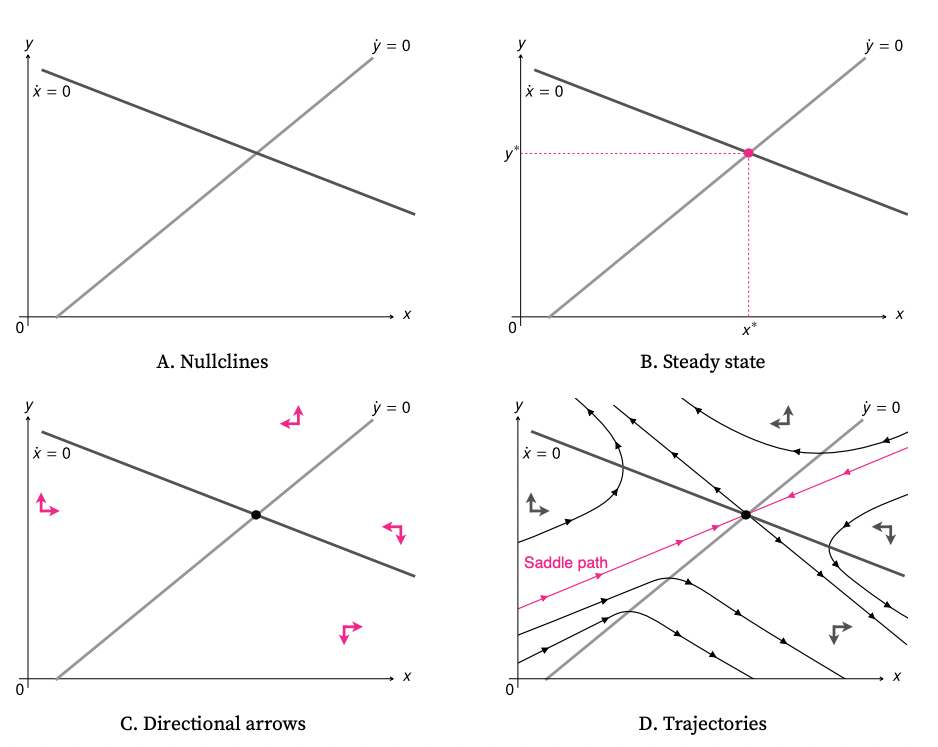
\includegraphics[scale=0.28]{figs/phasediag.png}
		\caption{Phase diagram of the dynamical system \eqref{phase_sys} \citep{michaillat2023} .}
		\label{fig:exmaple_phase}
	\end{figure}
	\end{frame}

	\begin{frame}{Example of a Nonlinear case: Optimal Growth}
	Given the system
	\begin{align}
		\begin{matrix}
			\dot{k} = f (k) - c - \delta k, \\
			\dot{c} = [ f'(k) - (\delta + \rho) ] c
		\end{matrix} \label{eq:sys_nonlin}
	\end{align}
		\begin{figure}[ht]
		\centering
			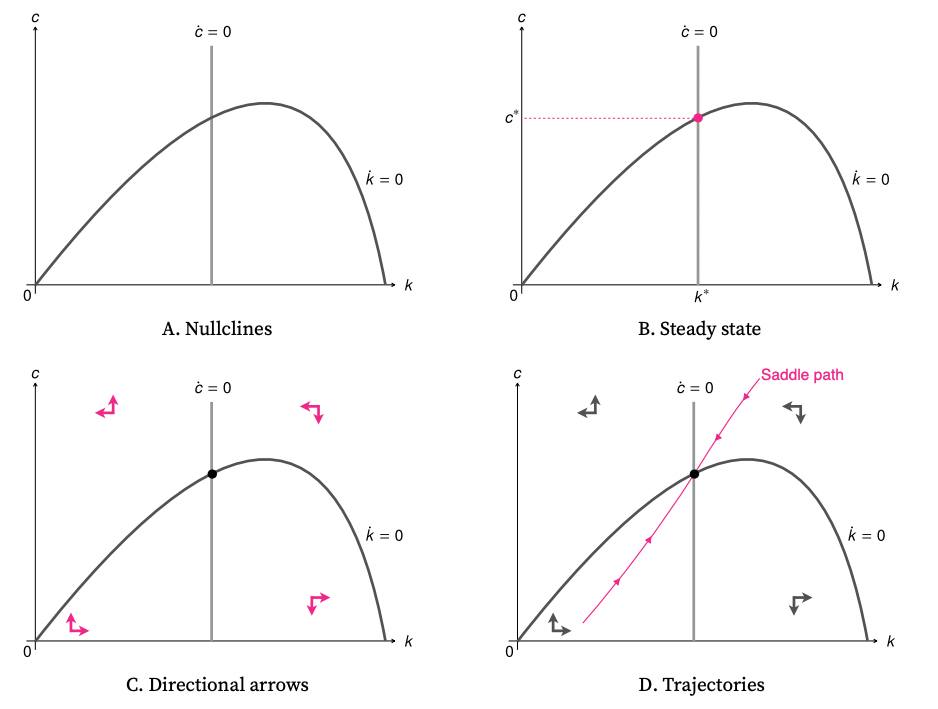
\includegraphics[scale=0.2]{figs/phasediag2.png}
		\caption{Phase Diagram of system \eqref{eq:sys_nonlin} \citep{michaillat2023}. }
		\label{fig:exmaple_phase}
	\end{figure}
	\end{frame}

\section{Dynamic Optimization}
\subsection{Dynamic Programming with Bellman}
\begin{frame}
	\frametitle{Dynamic Programming}
	\begin{align*}
		\max_{c_t} & \sum^\infty_{t=0}  \beta^t u(c_t) \\
		&(\textbf{transition equation}) & k_{t+1} &= f(k_t) + (1-\delta)k_t - c_t, \\
		&(\textbf{initial condition}) & k_0 &> 0 \\
		&(\textbf{transversality condition)} & \lim_{t\to 0} & \beta^t u'(c_t) k_{t+1} = 0
	\end{align*}
\begin{enumerate}
\item Write the Bellman equation
		\begin{align}
			V(k_t) =  \left[ u(c_t) + \beta V(k_{t+1}) \right] \label{eq:bellman}
		\end{align}
\item Solve for policy function by maximizing $V$ with respect to control variable
\begin{align*}
			\frac{\partial V(k_t)}{\partial k_{t+1}} = 0 \Leftrightarrow \frac{\partial u(k_{t+1})}{\partial k_{t+1}} + \beta \blue{\frac{\partial V(k_{t+1})}{\partial k_{t+1}}} = 0 
		\end{align*}
\item Use Benveniste-Scheinkman Equation for $\frac{\partial V(k_t)}{\partial k_t}$ then forward to $t+1$.
\item Obtain Euler: $\frac{u'(c_t)}{u'(c_{t+1})} = \beta (f'(k_{t+1}) + (1-\delta))$. Policy function maps $k_t$ to $c_t$.
\end{enumerate}
\end{frame}

\begin{frame}
	\frametitle{Dynamic Programming}
	Further issues
	\begin{enumerate}
		\item How to obtain the closed-form Value function and Policy function?
		\item Value function iteration algorithm.
		\item Steady state
		\item Stability of the steady state
	\end{enumerate}
\end{frame}

\subsection{Optimal Control with Hamiltonian}
\begin{frame}
	\frametitle{Optimal Control}
	We want to $\max_{ \{c_t\}^T_{t=0} } e^{-(\rho-n) t} u(c_t)  dt$
	\begin{align*}
		&(\textbf{transition equation}) & \dot{k}_t &= f(k_t) - \delta k_t - c_t, \\
		&(\textbf{initial condition}) & k_0 &> 0 \\
		&(\textbf{transversality condition}) & \lim_{t\to\infty} &\lambda_t k_t = 0
	\end{align*}
	The control variable is $c_t$, and the state variable is $k_t$.
	\begin{enumerate}
		\item Write the present-value Hamiltonian
		\begin{align*}
			H_t = u(c_t)e^{-\rho t} + \lambda_t (\dot{k}_t)
		\end{align*}
		\item Take FOC wrt to control variable
		\begin{align*}
			\frac{\partial H_t}{\partial c_t} = 0 \Leftrightarrow e^{-\rho t} u'(c_t) = \lambda_t.
		\end{align*}
		\item Take FOCs wrt to the state and co-state variable
		\begin{align*}
			\dot{k}_t = \frac{\partial H_t}{\partial \lambda_t} = f(k_t) - c_t - \delta k_t, &&
			\dot{\lambda}_t = \red{-} \frac{\partial H_t}{\partial k_t} = - \lambda_t (f'(k_t) - \delta)
		\end{align*}
		\item Derive the Euler equation by diff. control FOC wrt time. $\frac{\dot{c}_t}{c_t} = f'(k_t) - \delta - \rho. $
	\end{enumerate}
\end{frame}

%\section{Brownian Motion and Martingales}
%
%\begin{frame}
%\frametitle{Brownian Motion and Martingales}
%
%\textbf{Section: Brownian Motion}
%
%\begin{itemize}
%  \item \textbf{Standard Brownian Motion (Wiener Process):}
%    \begin{itemize}
%      \item Stochastic process $\{W_t, t \geq 0 \}$ with properties:
%      \item $W_0 = 0$
%      \item Independent increments
%      \item Gaussian increments: $W_t - W_s \sim N(0, t-s)$
%      \item Continuous sample paths, no jumps
%      \item Stationary increments
%    \end{itemize}
%  
%  \item \textbf{Statistical properties:}
%    \begin{itemize}
%      \item $E(W_t) = 0$
%      \item $Var(W_t) = t$
%      \item $Cov(W_s, W_t) = \min(s,t)$
%      \item $Corr(W_s, W_t) = \sqrt{\frac{\min(s,t)}{\max(s,t)}}$
%    \end{itemize}
%  
%  \item \textbf{General Brownian Motion:}
%    \begin{itemize}
%      \item With drift parameter $\mu$ and volatility $\sigma$
%      \item $X_t = X_0 + \mu t + \sigma W_t$
%    \end{itemize}
%\end{itemize}
%
%\end{frame}
%
%
%\begin{frame}
%\frametitle{Brownian Motion and Martingales (cont'd)}
%
%\textbf{Section: Brownian Motion (cont'd)}
%
%\begin{itemize}
%  \item \textbf{Geometric Brownian Motion:}
%    \begin{itemize}
%      \item $S_t = e^{X_t} = S_0 e^{\mu t + \sigma W_t}$
%    \end{itemize}
%
%  \textbf{Section: Martingales}
%  
%  \item \textbf{Discrete Time Martingales:}
%    \begin{itemize}
%      \item Stochastic process $\{X_n\}$
%      \item Martingale properties...
%    \end{itemize}
%    
%  \item \textbf{Filtration:}
%    \begin{itemize}
%      \item Collection of $\sigma$-algebras $\{F_t\}$
%      \item Adaptivity, information accumulation, independence...
%    \end{itemize}
%    
%  \item \textbf{Continuous Time Martingales:}
%    \begin{itemize}
%      \item Stochastic process $\{X_t\}$
%      \item Adapted to filtration, expected change is zero...
%    \end{itemize}
%\end{itemize}
%\end{frame}
%
%\section{Stochastic Calculus and Ito Process}
%
%\begin{frame}
%\frametitle{Stochastic Calculus and Ito Process}
%
%\textbf{Stochastic Calculus} is a branch of mathematics that deals with operations on stochastic processes. It provides a consistent theory of integration for stochastic processes and helps describe continuous-time processes using stochastic differential equations (SDE).
%
%\textbf{Ito Integral}
%
%\begin{itemize}
%  \item Ito integral: $\int_a^b C_s dW_s$
%  \item Direct approach fails due to non-differentiability and unbounded variation of $W_t$
%  \item Ito integrals defined through step function approximations
%\end{itemize}
%
%\end{frame}
%
%\begin{frame}
%\frametitle{Ito Process and Ito Formula}
%
%\textbf{Geometric Brownian Motion Revisited}
%
%\begin{itemize}
%  \item Geometric Brownian Motion: $S_t = S_0 e^{(\alpha - 0.5 \sigma^2)t + \sigma W_t}$
%  \item Drift parameter $\mu = \alpha - \frac{1}{2}\sigma^2$, diffusion parameter $\sigma$
%  \item Solution of SDE: $\frac{S_t}{S_0} \sim \text{LogN}((\alpha - \frac{1}{2}\sigma^2)t, \sigma^2 t)$
%\end{itemize}
%
%\textbf{Mean-Reverting Process}
%
%\begin{itemize}
%  \item Spot rate of interest model: $dr_t = -\alpha (r_t - \mu)dt + \sigma dW_t$
%  \item SDE: $dX_t = -\alpha X_t dt + \sigma dW_t$
%  \item Solution: $X_t = X_0 e^{\alpha t} + \sigma e^{-\alpha t} \int_0^t e^{\alpha s} dW_s$
%\end{itemize}
%
%\end{frame}
%
%\section{Derivative Securities}
%\begin{frame}
%\frametitle{Introduction to Derivative Securities}
%A derivative security is a financial contract whose value is derived from another underlying security.
%\begin{itemize}
%    \item Underlying securities: stock, bond, index, currency, etc.
%    \item Common derivatives: Forwards, Futures, Options, Swaps
%\end{itemize}
%
%\textbf{Forward Contract}: Agreement to buy/sell an asset at a future date for a pre-agreed price.
%
%\textbf{Futures Contract}: Standardized forward contract traded on an exchange.
%
%\textbf{Option}: Conveys the right (not obligation) to transact at a future date.
%\begin{itemize}
%    \item Call: Right to buy
%    \item Put: Right to sell
%    \item European: Exercise at maturity
%    \item American: Exercise anytime until maturity
%\end{itemize}
%\end{frame}
%
%\begin{frame}
%\frametitle{Introduction to Derivative Securities}
%\textbf{Assumptions}:
%\begin{itemize}
%    \item No market frictions, competitive markets, rational agents
%    \item No arbitrage (no-risk profit)
%\end{itemize}
%
%\textbf{Forward Contracts}:
%\begin{itemize}
%    \item $F_{0,T} = S_0 e^{rT}$ for non-dividend-paying share
%    \item $F_{0,T} = (S_0 - I) e^{rT}$ for discrete dividend-paying share
%    \item $F_{0,T} = S_0 e^{(r-q)T}$ for continuous dividend-paying share
%    \item $F_{0,T} = S_0 e^{(r-r_e)T}$ for currency exchange
%    \item Biased predictor of the future spot price
%\end{itemize}
%
%\textbf{Hedging with Futures}:
%\begin{itemize}
%    \item Long/short hedge: manage market risk
%    \item Basis risk: hedging with different assets
%    \item Optimal hedge ratio
%\end{itemize}
%\end{frame}
%
%\section{Binomial Model Overview}
%\begin{frame}
%\frametitle{Binomial Model Overview}
%In the binomial model for option pricing:
%\begin{itemize}
%\item Stock price follows a discrete-time stochastic process.
%\item Binomial trees (lattices) are used.
%\item The no-arbitrage principle and risk-neutral pricing are applied.
%\item Key concepts of financial pricing are introduced.
%\item The Black-Scholes model is a limiting case.
%\end{itemize}
%
%Two tradeable assets: risky asset (stock) and riskless asset (cash).
%\begin{itemize}
%\item Stock price process: $S_t$, $S_{t+1} = \begin{cases} uS_t, \text{ with probability } p \\ dS_t, \text{ with probability } 1-p \end{cases}$.
%\item Cash process: $B_t$, $B_t = e^{rt}$.
%\end{itemize}
%\end{frame}
%
%\begin{frame}
%\frametitle{One-Period Model and Replicating Portfolio}
%\textbf{One-Period Model:}
%\begin{itemize}
%\item Stock price moves up to $uS_0$ or down to $dS_0$.
%\item Option payoff: $f_u$ for up move, $f_d$ for down move.
%\end{itemize}
%
%\textbf{Replicating Portfolio:}
%\begin{itemize}
%\item Construct a portfolio $(\phi, \psi)$ of stock and cash.
%\item Portfolio value at time 1: $\phi uS_0 + \psi e^r$ or $\phi dS_0 + \psi e^r$.
%\item Choose $\phi$ and $\psi$ to match option payoff.
%\item No-arbitrage principle leads to option price formula.
%\end{itemize}
%
%\textbf{Risk-Neutral Pricing:}
%\begin{itemize}
%\item Option price: $f_0 = e^{-r}[qf_u + (1-q)f_d]$.
%\item $q$ is risk-neutral probability of an up move.
%\item Option price is discounted expected payoff under risk-neutral measure.
%\end{itemize}
%\end{frame}



	%----------------------------------------------------------------------------------------
	%	BIB
	%----------------------------------------------------------------------------------------

	
	
\end{document}